\begin{figure}[h]
\def\vertspace{1ex}
\rotatebox{90}{\hspace{1ex}\tiny Square map}%
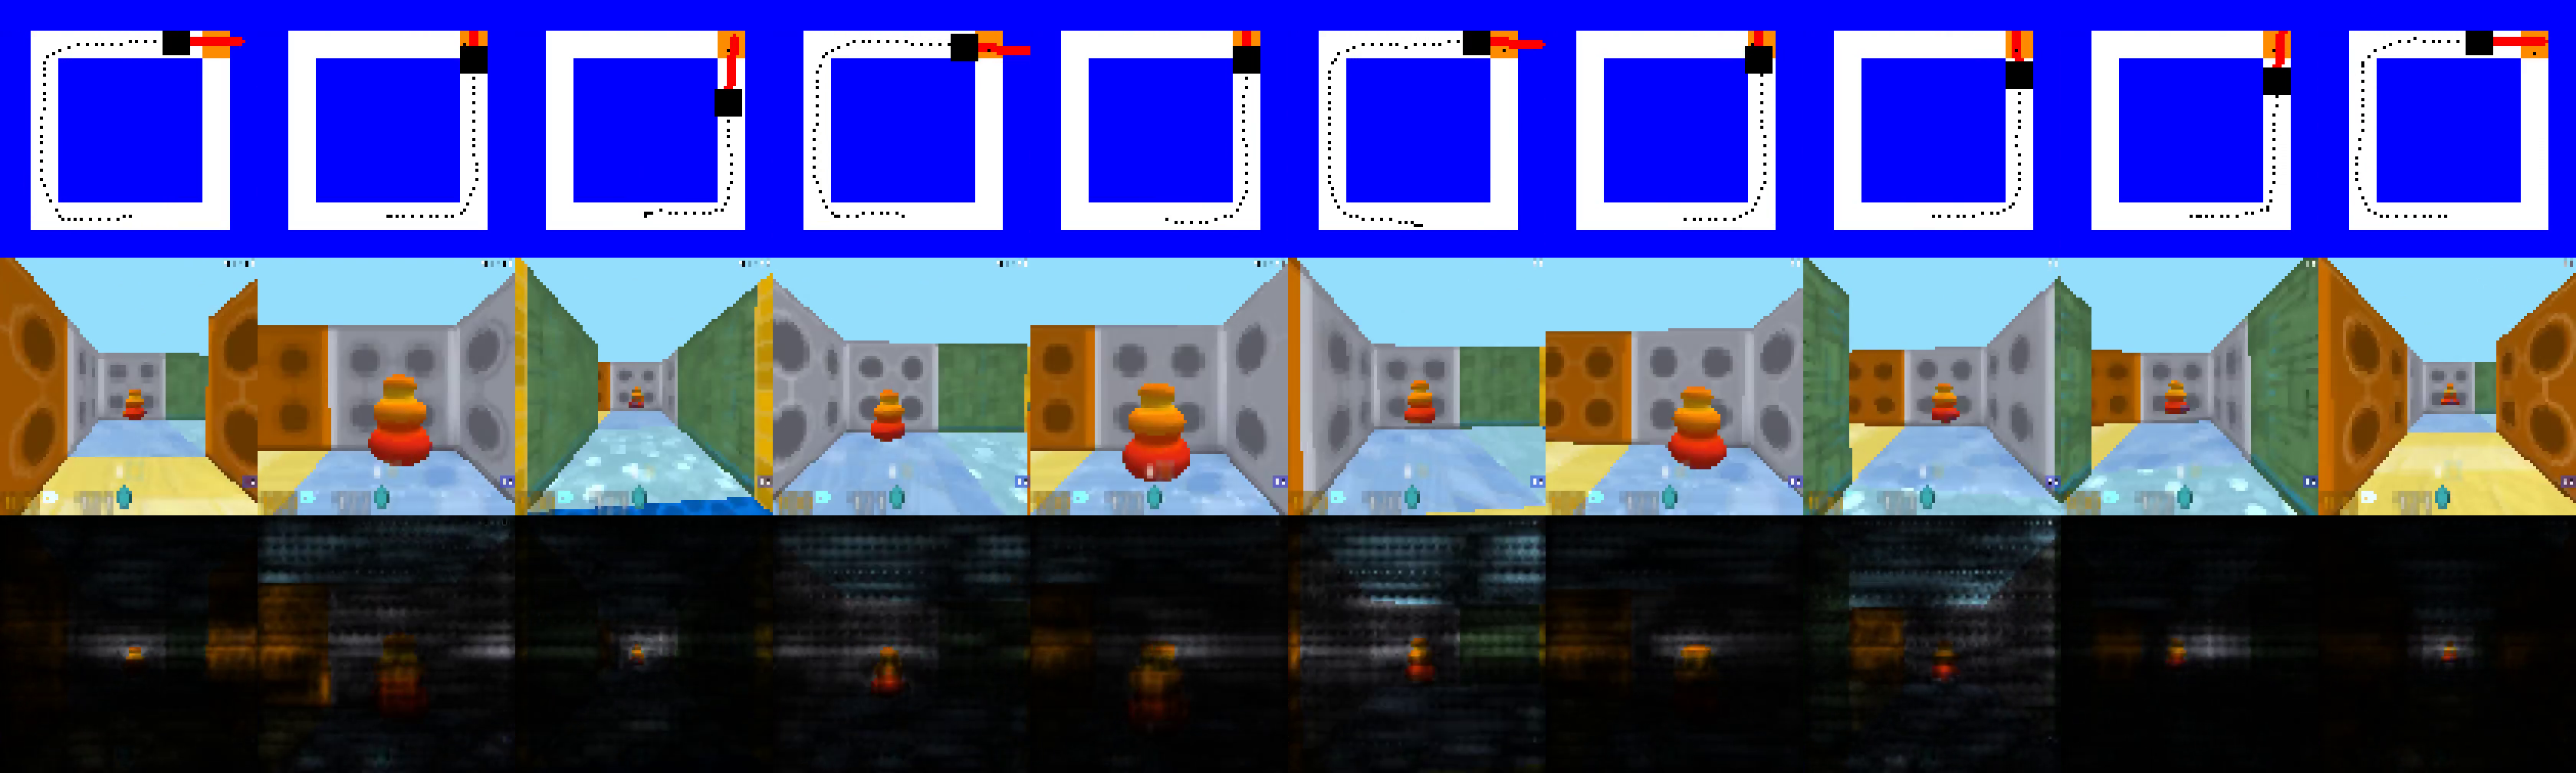
\includegraphics[width=0.98\textwidth,trim=0 672pt 0 0,clip]{./exp-results/training-1000_on_square_map.png}%
\vspace{\vertspace}
\rotatebox{90}{\hspace{1ex}\tiny Wrench map}%
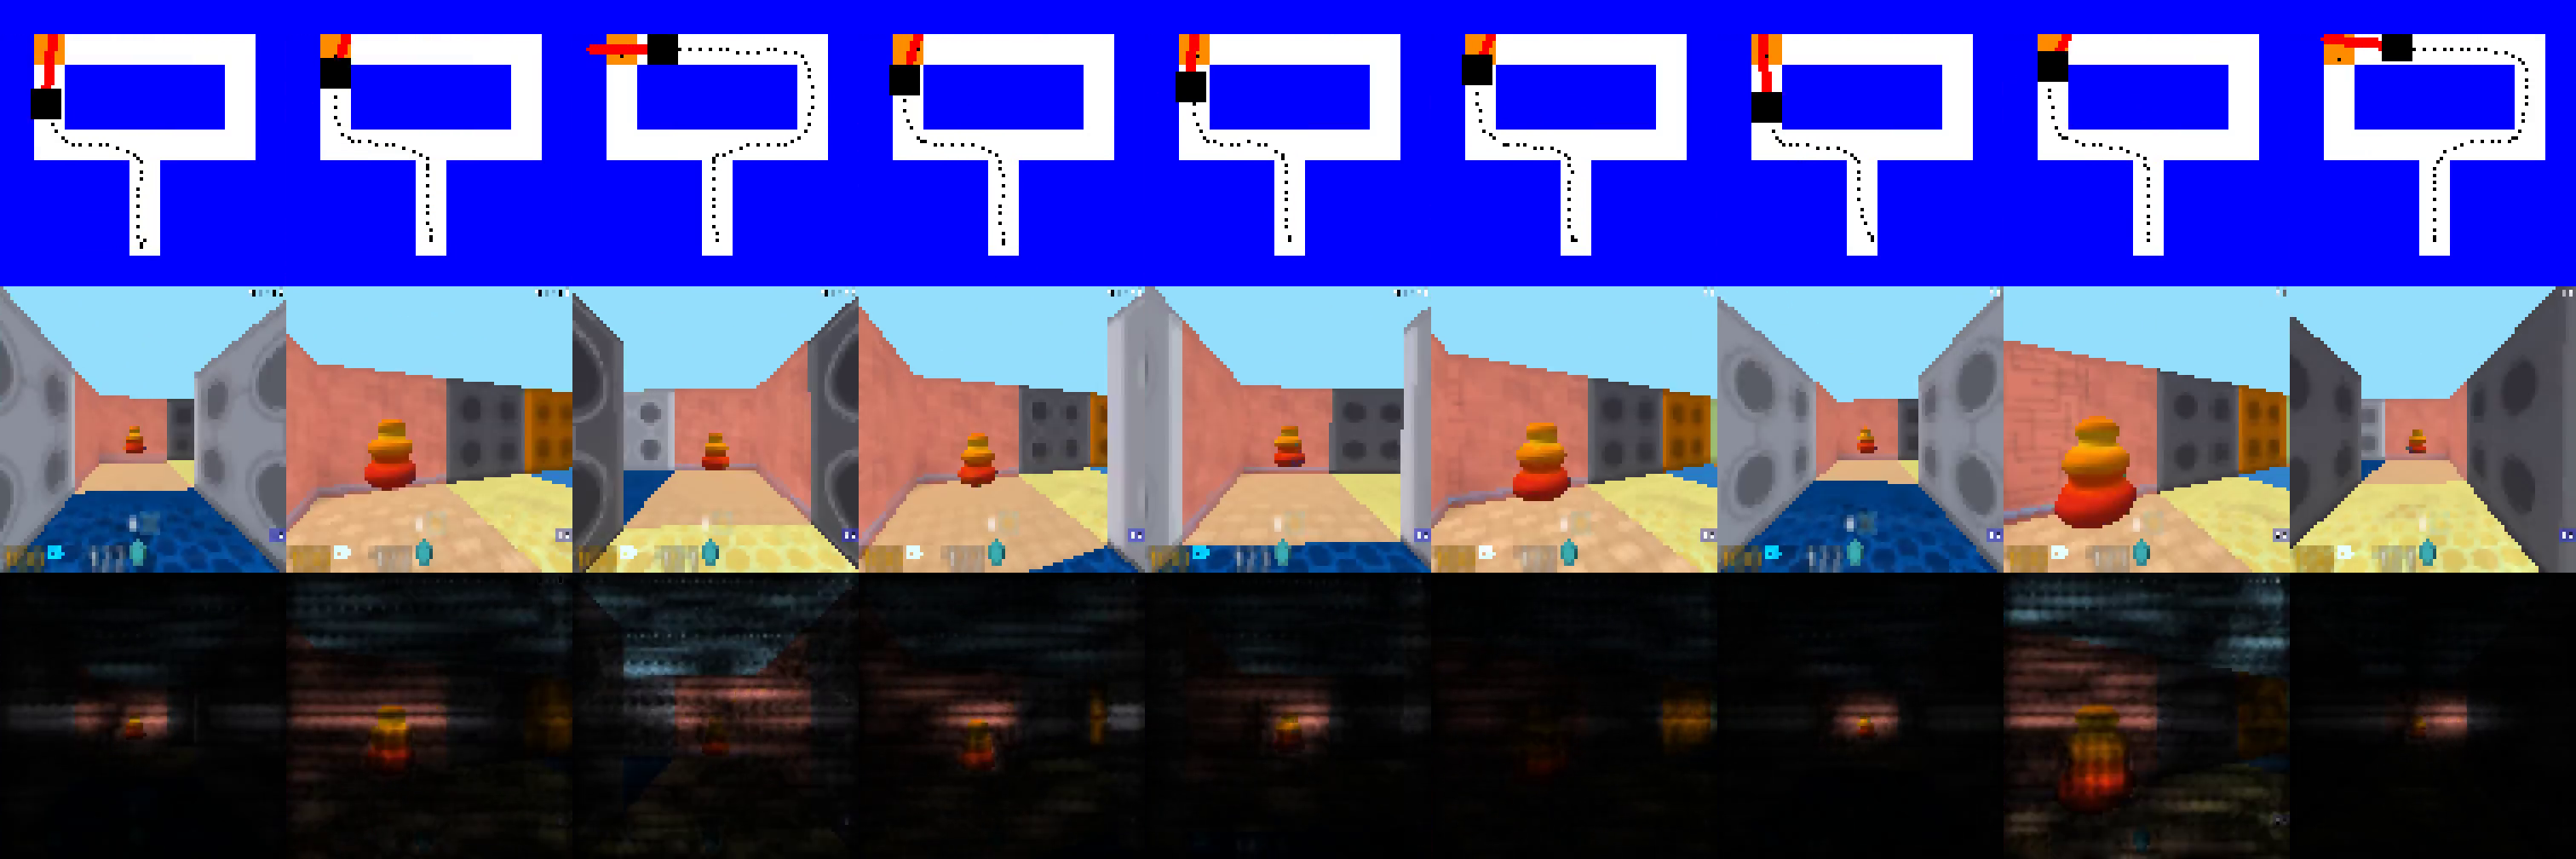
\includegraphics[width=0.98\textwidth,trim=0 672pt 0 0,clip]{./exp-results/training-1000_on_wrench_map.png}%
\vspace{\vertspace}
\rotatebox{90}{\hspace{2ex}\tiny Goal map}%
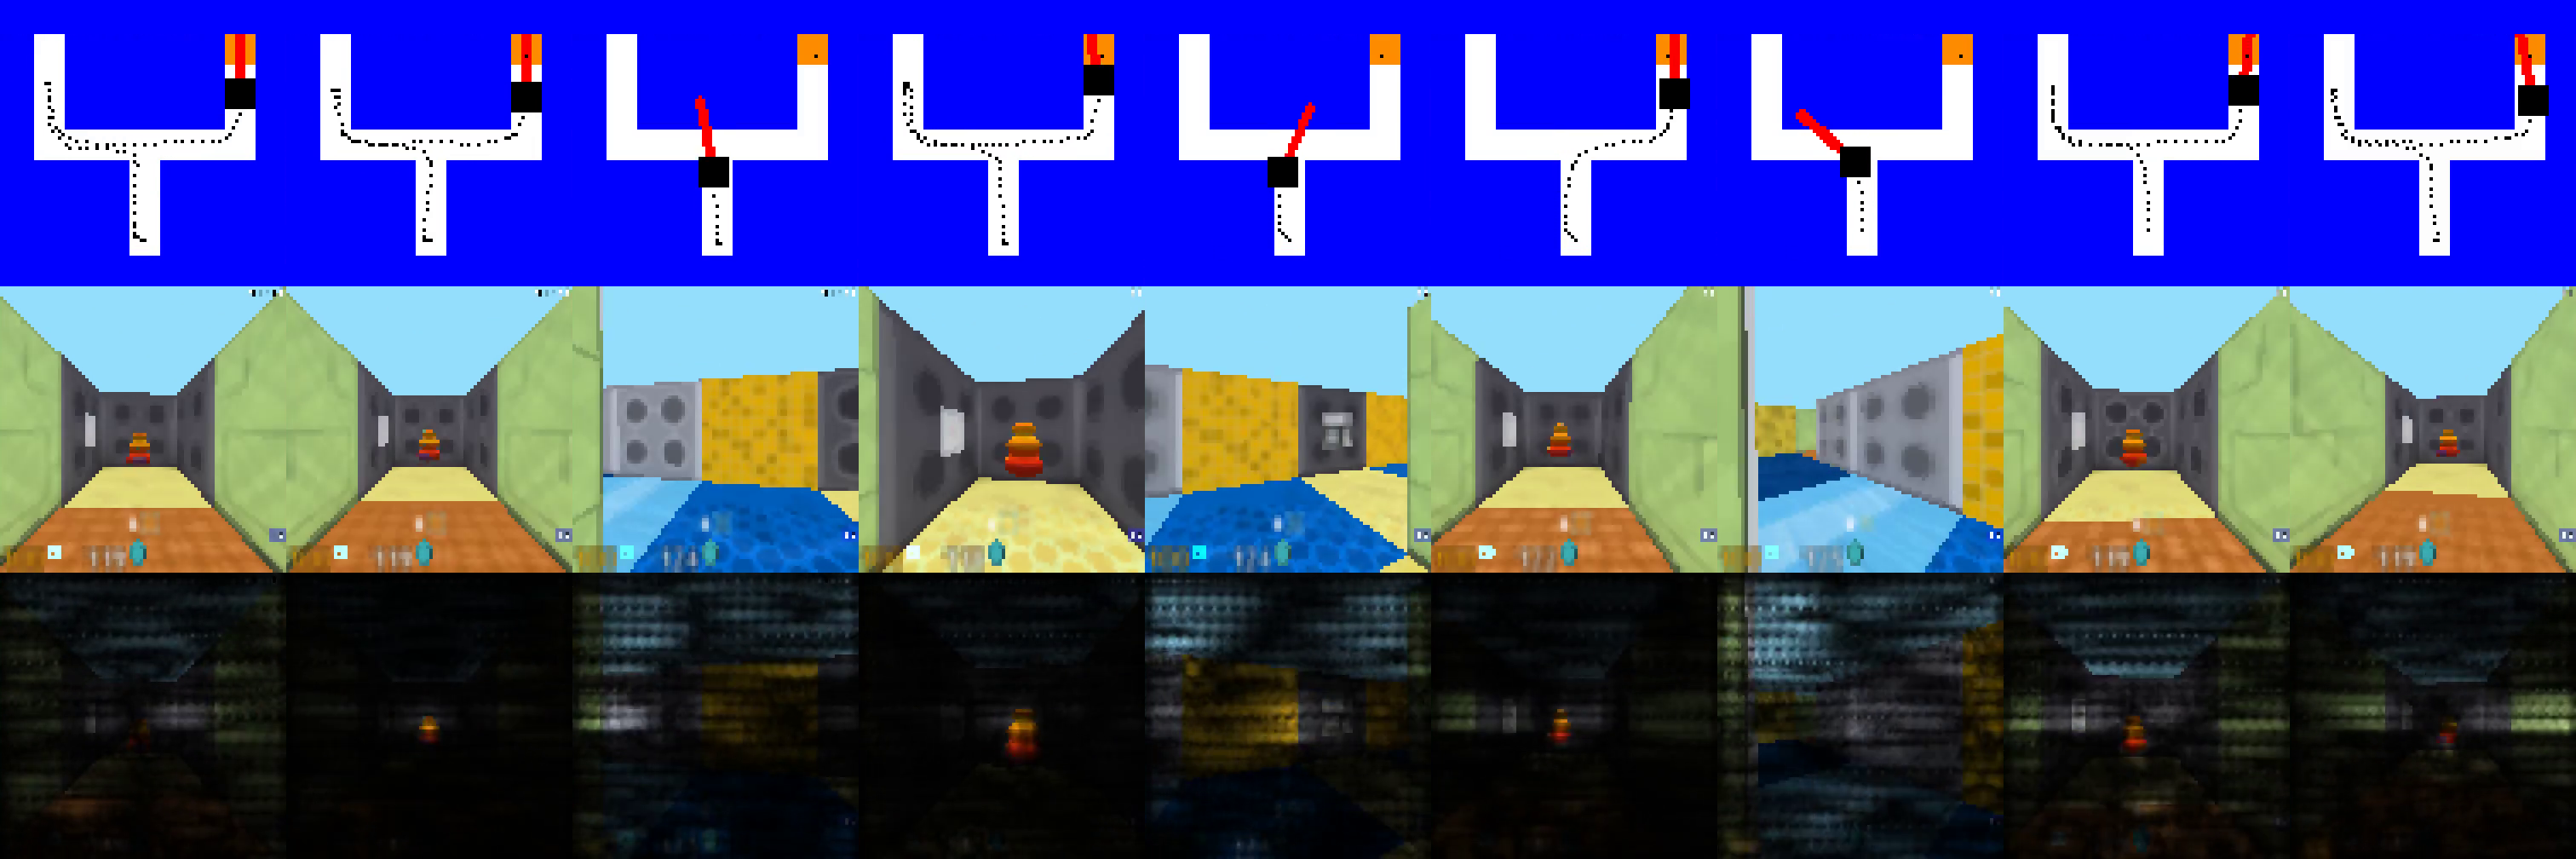
\includegraphics[width=0.98\textwidth,trim=0 672pt 0 0,clip]{./exp-results/training-1000_on_goal_map.png}%
\caption{Snapshots of path taken by the agent to reach the goal in a single episode when model trained on 1000 maps is evaluated Square, Wrench and Goal map.
  The top row shows an evaluation example on Square map, the agent takes the shortest path 6/10 times but when averaged over 100 episodes, the percentage of shortest path taken is not better than random $50.4$\% ($\pm 12.8$\%).
  Although for the example of Wrench map the agent takes the shortest path 8/10 times but when averaged over 100 episodes, the percentage of shortest path taken is reduced to $32.9$\% ($\pm 25.1$\%).
 For the Goal map, the example chosen here shows that the shortest path is only taken 1/6 times, on an average over 100 episodes, the shortest path is taken $42.6$\% ($\pm 35.1$\%) times.
}
\label{fig:planning-qualitative}
\end{figure}
